\section{Semi-open Rail Waiting Areas: Revising the Bus Model}
\label{sec:rail}

Requirement 2(b) retains the service objective, but changes how local conditions are obtained. A roof and partial walls permit air and surface temperatures to retain a history of earlier loads. Evaporative devices can humidify recirculated air, while passengers and outdoor exchange vary over a train cycle. We therefore replace prescribed temperature/humidity fields with a three-zone dynamic control-volume model. The zones represent the entrance, waiting core, and platform edge; they need not share the same conditions.

\begin{table}[!ht]
\centering\small
\caption{Revisions to the bus model and their purpose.}
\label{tab:rail-changes}
\begin{tabularx}{\linewidth}{@{}>{\raggedright\arraybackslash}p{0.25\linewidth}>{\raggedright\arraybackslash}X>{\raggedright\arraybackslash}X@{}}
\toprule
Revision & Why it is needed & Added capability\\
\midrule
Air and surface storage & Partial enclosure allows thermal memory. & Predict warm-up, lag and residual heat.\\
Dynamic moisture and zone exchange & Recirculation changes inlet humidity; openings connect different regions. & Calculate evaporative feedback and dilution.\\
Time-dependent passengers & Arrivals and boarding change both loads and service demand. & Count time-resolved person-hours and crowd heat/moisture.\\
All devices and their heat & Several units consume power and release heat within the station. & Use total electricity and include local dissipation.\\
\bottomrule
\end{tabularx}
\end{table}

\subsection{Coupled heat, moisture, and surface balances}

Following the control-volume structure of building heat and moisture balances \cite{epzone}, let each zone store moist-air enthalpy $h_z$ (J/kg dry air), humidity ratio $w_z$ (kg/kg dry air), and an effective roof/wall inner-surface temperature $T_{m,z}$. The air is well mixed within each zone. Its dry-air mass is approximated as constant, $M_z=\rho_{da,o}V_z$, with outdoor reference density. This is a reduced model, not an EnergyPlus or CFD simulation.

Define the exchange operator, for either $x=h$ or $w$, as
\begin{equation}
 \mathcal L_z(x)=\dot m_{0z}(x_o-x_z)+\sum_{j\ne z}\dot m_{zj}(x_j-x_z),
 \qquad \dot m_{0z}=M_z\lambda_z/3600.
\label{eq:rail-exchange}
\end{equation}
Here $\lambda_z$ is the assumed outdoor air-change rate in h$^{-1}$. Each exchange represents equal entering and leaving dry-air flow; adjacent-zone rates satisfy $\dot m_{zj}=\dot m_{jz}$. Wind, buoyancy and opening geometry can affect outdoor exchange \cite{ventilation}; a prescribed train-cycle pulse tests that uncertainty without claiming a station-specific piston-flow law.

With time in seconds, our balances are
\begin{align}
 M_z\dot h_z={}&\mathcal L_z(h)+H_{ma,z}(T_{m,z}-T_z)
 +n_zq_c+n_zg h_v(T_z)+P_z
 +\dot m_{e,z}(h_{e,z}-h_z),\label{eq:rail-enthalpy}\\
 M_z\dot w_z={}&\mathcal L_z(w)+n_zg+
 \dot m_{e,z}(w_{e,z}-w_z),\label{eq:rail-moisture}\\
 C_{m,z}\dot T_{m,z}={}&H_{mo,z}(T_o-T_{m,z})+Q_{\mathrm{sol},z}
 +n_zq_r-H_{ma,z}(T_{m,z}-T_z).\label{eq:rail-surface}
\end{align}
The per-person inputs are convective heat $q_c$, radiative heat $q_r$, and water-vapor generation $g$. Vapor enters with $h_v(T)=2501000+1860T$ J/kg; no additional latent-heat term is added. All device power $P_z$ is assumed to dissipate locally as sensible heat. Pump power is already included in the device total. Conductances $H$ have units W/K, surface capacity $C_m$ has units J/K, and $Q_{\mathrm{sol}}$ is an effective absorbed envelope load. The opposite signs of the air--surface term conserve internal energy.

Air temperature is recovered from $T_z=(h_z-2501000w_z)/(1006+1860w_z)$. A shaded longwave approximation for the surface contribution to comfort \cite{thermalcomfort} gives
\begin{equation}
 T_{r,z}=\left[F_z(T_{m,z}+273.15)^4+(1-F_z)(T_{r,o}+273.15)^4\right]^{1/4}-273.15.
\label{eq:rail-mrt}
\end{equation}
$F_z$ is an assumed effective view fraction; the example sets external radiant temperature $T_{r,o}=T_o$, while keeping it a separate input. Direct sun on passengers and detailed radiative asymmetry are excluded.

\noindent\textbf{Device mechanisms.} A adds air movement and electrical heat, with $\dot m_e=0$. B/C recirculate local air: at every step Eq.~\eqref{eq:outlet} is evaluated using the \emph{current zone inlet}, rather than fixed outdoor conditions. Their approximate outlet enthalpy remains $h_{e,z}=h_z$, while $w_{e,z}>w_z$ when evaporation occurs. Thus evaporation can lower dry-bulb temperature without removing moist-air enthalpy. Rising local moisture reduces subsequent wet-bulb depression. The earlier fixed mixing fractions are replaced by these explicit flow balances. Local passenger air speeds remain stated assumptions, rather than solutions of a momentum model.

\subsection{A matched, reproducible station scenario}

We use an illustrative $24\times10\times4$ m waiting area, divided along its length into three $80\,\mathrm{m^2}$ zones of $320\,\mathrm{m^3}$ each. These are scenario dimensions, not measurements of a named station. Outdoor temperature is $33\,^{\circ}\mathrm C$, with RH $30\%$ and $70\%$. SET retains the bus model's $1.2$ met, $0.5$ clo, and common $26\,^{\circ}\mathrm C$ reference.

\begin{table}[!ht]
\centering\small
\caption{Explicit rail-scenario assumptions; zone vectors follow entrance/core/platform order.}
\label{tab:rail-inputs}
\begin{tabularx}{\linewidth}{@{}>{\raggedright\arraybackslash}p{0.29\linewidth}>{\raggedright\arraybackslash}X@{}}
\toprule
Input & Assumed value\\
\midrule
Train cycle and passengers & Every 15 min, $n_z$ rises linearly from $(6,10,4)$ toward $(20,45,15)$, then resets after boarding.\\
Outdoor and zone exchange & Base $\lambda=(8,4,10)$ h$^{-1}$; add $(8,4,12)$ h$^{-1}$ in the final 2 min of each cycle. Adjacent zones exchange $0.20$ kg dry air/s.\\
Surface response, each zone & $C_m=4.0$ MJ/K, $H_{ma}=200$ W/K, $H_{mo}=400$ W/K, $Q_{\mathrm{sol}}=800$ W; $F=(0.55,0.85,0.55)$.\\
Per-person sources & $q_c=45$ W, $q_r=30$ W, $g=45/(2.45\times10^6)$ kg/s. Fixed representative loads, not measured passenger emissions.\\
Equipment count and power & One unit per zone: total $0.75/3.60/7.50$ kW for A/B/C. All three units run throughout the two-hour assessment.\\
Evaporative recirculation & B/C: $0.60/1.20$ kg dry air/s per zone; $\varepsilon=0.70$; outlet caps $5/8\,^{\circ}\mathrm C$.\\
Passenger air speeds & Baseline $0.20$ m/s; A $(0.60,1.00,0.50)$, B $(0.50,0.80,0.45)$, C $(0.75,1.00,0.60)$ m/s.\\
\bottomrule
\end{tabularx}
\end{table}

The three sources of information remain separate: powers and nominal effect descriptions come from the problem, balance mechanisms come from the cited literature, and the station geometry, flows, loads and schedules are assumptions. We do not fit them to obtain a preferred device ranking.

Each climate--exchange case first receives a prescribed two-hour uncooled warm-up from outdoor air and surface conditions. All strategies then start from that \emph{same} warm-up state and are assessed for two hours. The independent no-device trajectory uses identical passengers, weather and exchange. This specifies a common prior history; it is not a claim that a periodic steady state has been reached. It prevents stored cooling from being supplied free at the initial time. Later benefits beyond the assessment horizon are not credited.

\subsection{Service accounting and numerical findings}

For each strategy, compute $\Theta_{s,z}(t)$ from the evolving $(T_z,T_{r,z},v_{s,z},\mathrm{RH}_z)$, and retain the original signed accounting:
\begin{equation}
 \eta_s=\frac{\int_0^{2\mathrm{h}}\sum_z n_z(t)
 \{D[\Theta_{0,z}(t)]-D[\Theta_{s,z}(t)]\}\,dt}
 {\int_0^{2\mathrm{h}}\sum_z P_{s,z}(t)\,dt}.
\label{eq:rail-efficiency}
\end{equation}
Time in this integral is measured in hours and power in kW. The two-hour electricity totals are $1.5$, $7.2$, and $15.0$ kWh. Average remaining discomfort is reported alongside efficiency, so high passenger throughput cannot substitute for adequate local relief. The baseline ratio is undefined because its active-cooling energy is zero.

\begin{figure}[!ht]
\centering
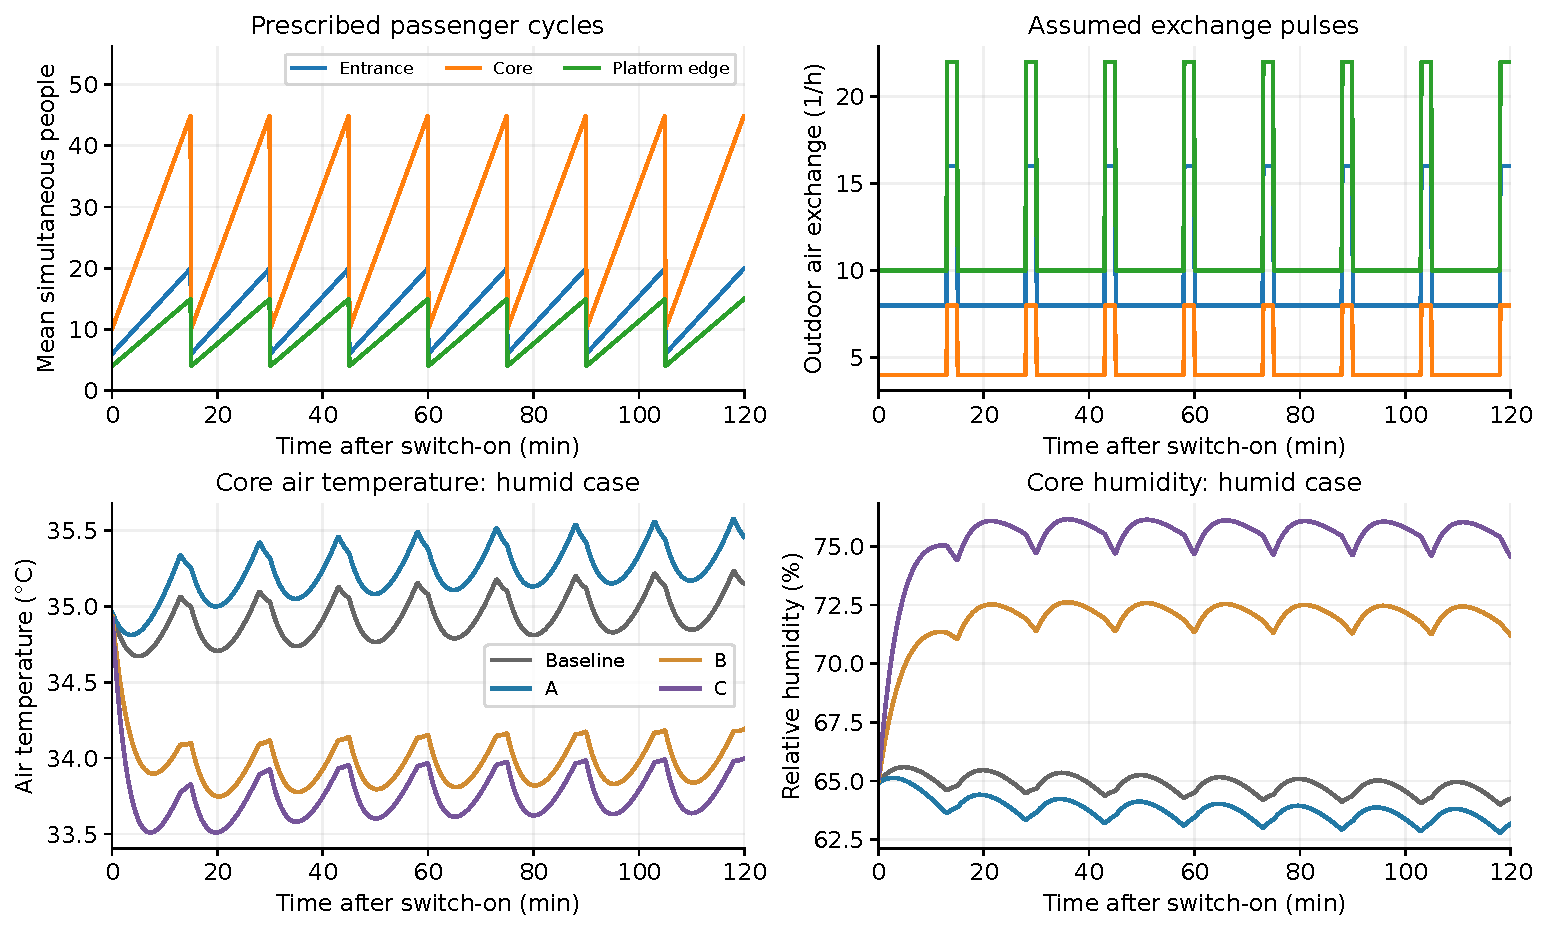
\includegraphics[width=\linewidth]{figures/10_rail_dynamics.pdf}
\caption{Assumed passenger/air-exchange cycles and simulated waiting-core temperature and RH in the humid rail scenario. The device cases and uncooled baseline start from the same state.}
\label{fig:rail-dynamics}
\end{figure}

The evaluation contains $100$ person-hours. In the dry case, A/B/C provide efficiencies of $145.9/35.6/26.1$ person$\cdot{}^{\circ}\mathrm C\cdot$h/kWh and mean remaining SET excesses of $3.62/3.24/1.90\,^{\circ}\mathrm C$. A uses electricity most efficiently, while C delivers the greatest average relief. In the humid case, efficiencies are $168.7/29.4/15.3$, and remaining excesses are $8.04/8.45/8.27\,^{\circ}\mathrm C$. Under these particular flows and loads, A also gives the lowest remaining discomfort. No case establishes adequate thermal protection merely by winning this comparison.

In the humid core, B and C reach RH peaks of $72.6\%$ and $76.2\%$, compared with $65.1\%$ for A. Figure~\ref{fig:rail-dynamics} exposes the evolving inlet conditions that a fixed outdoor-state calculation would miss. These rail results use different geometry, loads and delivery assumptions from the bus example; their differing rankings alone do not measure a gain in predictive accuracy.

\begin{figure}[!ht]
\centering
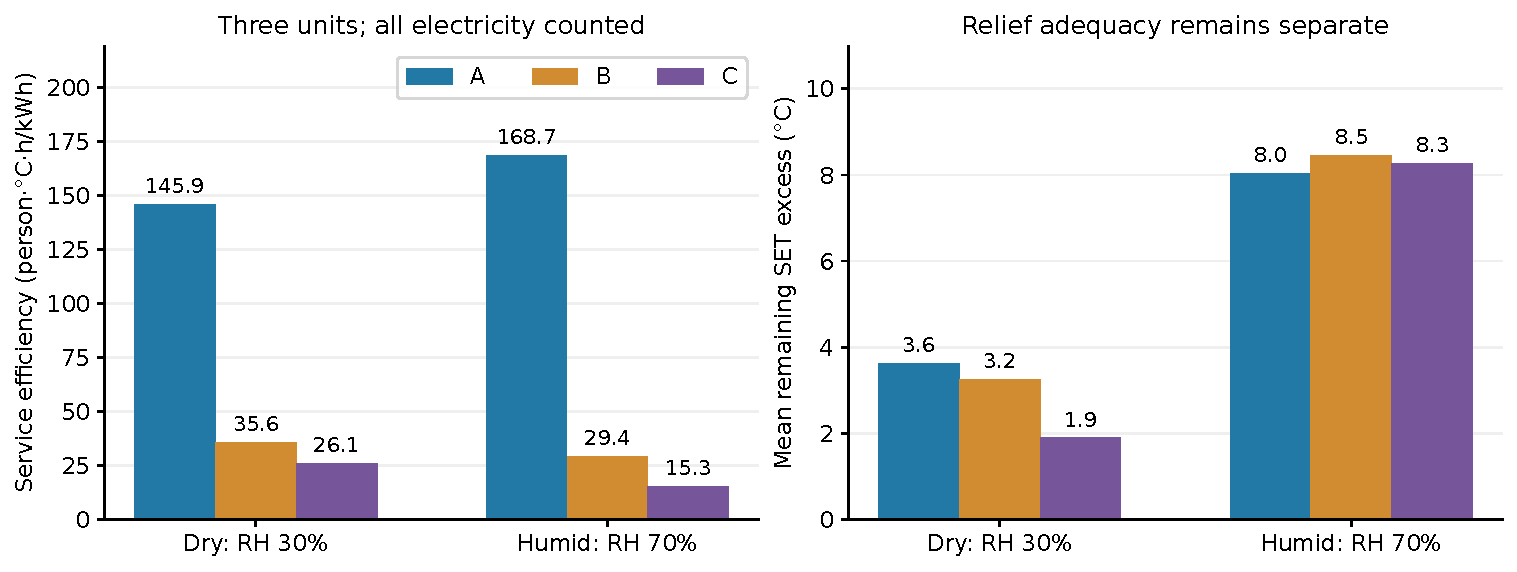
\includegraphics[width=\linewidth]{figures/11_rail_efficiency.pdf}
\caption{Rail-scenario service efficiency and mean remaining SET excess, with all three units' electricity included. Results are conditional simulations, not station measurements.}
\label{fig:rail-efficiency}
\end{figure}

\begin{figure}[!ht]
\centering
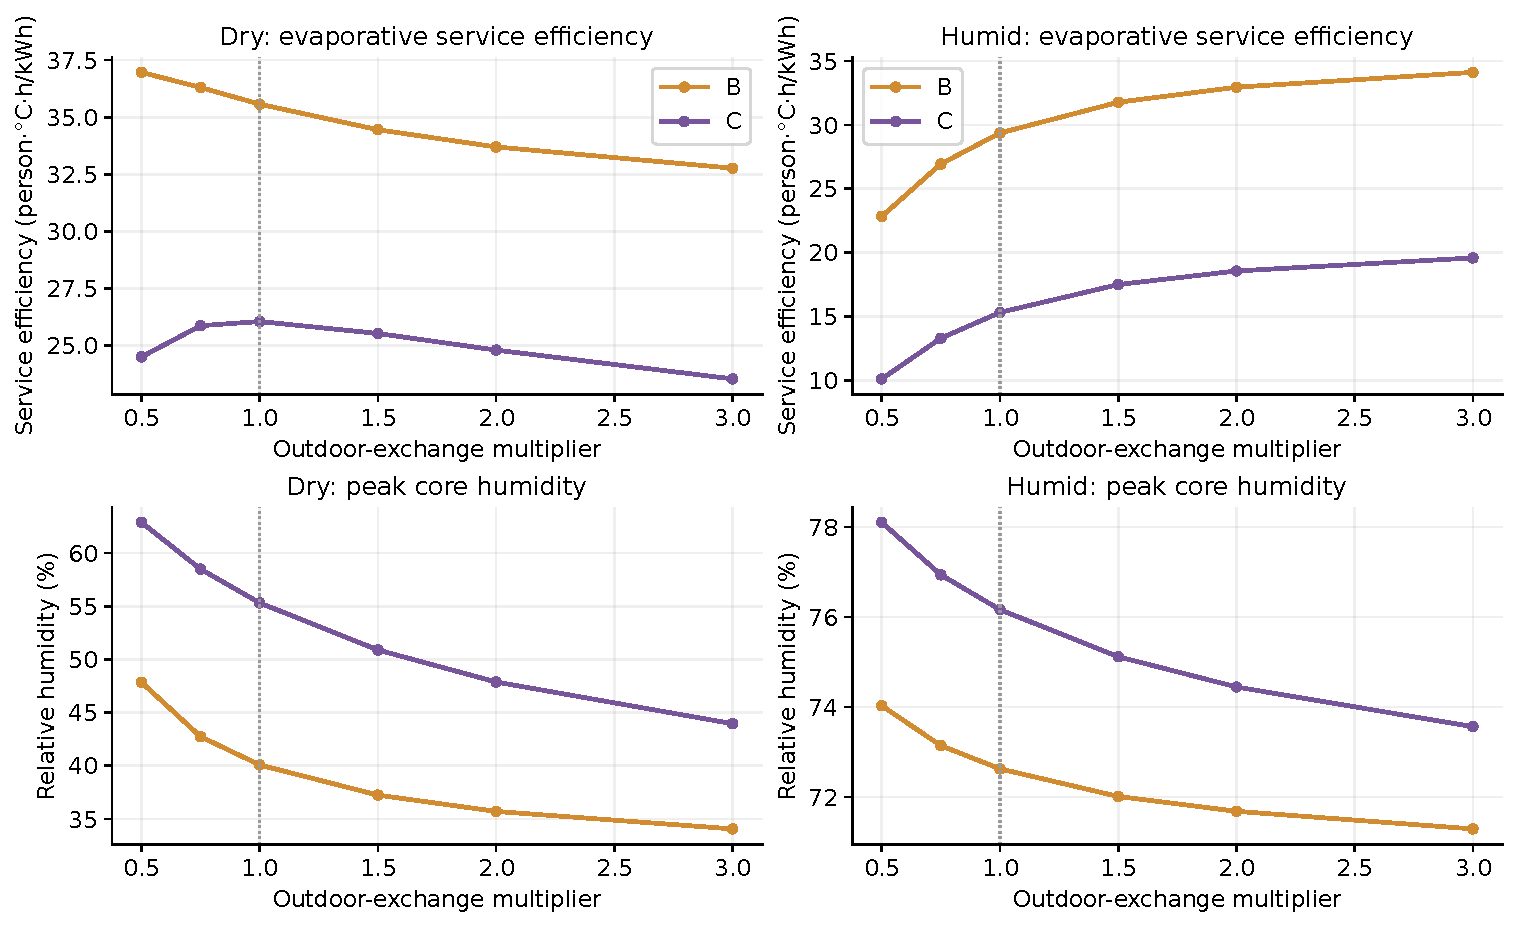
\includegraphics[width=\linewidth]{figures/12_rail_ventilation.pdf}
\caption{Outdoor-exchange sensitivity with equipment, local passenger air speeds and other inputs fixed. Each case uses its own matched uncooled baseline. The sweep isolates heat/moisture exchange; it does not predict a complete opening redesign.}
\label{fig:rail-ventilation}
\end{figure}

The exchange sweep shows competing effects. For dry-case C, efficiency at multipliers $0.5$, $1$, and $3$ is $24.5$, $26.1$, and $23.5$: more exchange removes retained moisture and heat but also dilutes cooling. The best of these sampled settings is not a universally optimal ventilation rate. For humid-case C, the same settings give $10.1$, $15.3$, and $19.6$, while mean remaining excess falls from $9.48$ to $8.27$ to $7.22\,^{\circ}\mathrm C$. Thus treating all outdoor exchange as waste would conceal a useful heat/moisture removal mechanism. Local air speeds remain fixed in this diagnostic sweep.

\subsection{What the revision improves, and what remains uncertain}

The revised model can evaluate when moisture accumulates, how the core differs from an exposed edge, and how a train-cycle crowd changes both thermal demand and useful service. It also makes finite air residence and surface thermal memory explicit. The bus model's fixed profiles could not resolve those histories. Consequently, the revision improves the \emph{questions the model can answer}; an improvement in field prediction accuracy still requires measured temperatures, RH, air speeds, surface temperatures, occupancy and electricity.

\Needspace{9\baselineskip}
\noindent\textbf{Verification.} The solver uses RK4 with a $10$ s step and midpoint schedule values; steps align with every pulse and boarding boundary. Halving the step changes efficiency by less than $0.001\%$ and mean remaining discomfort by less than $10^{-5}\,^{\circ}\mathrm C$ in all nominal cases. Checks close total air-plus-surface energy and water-vapor budgets, verify internal exchange cancellation, reproduce an unloaded equilibrium, and retain zero service at zero occupancy despite positive device electricity. The service identity $U_s+R_s=R_0$ also holds. These checks establish numerical consistency, not field accuracy.

The accompanying \texttt{station\_model} folder contains the scenario, solver, CSV trajectories, initial states, sensitivity results and verification records. SET remains a quasi-steady human-response calculation even though the environment is dynamic. The model neglects surface moisture sorption, condensation, detailed stratification and direct solar exposure. It stops on invalid humidity or SET inputs instead of hiding them. Outdoor exchange and local air speeds need field calibration before operational recommendations; the exchange sweep is a thermal comparison, not a ventilation or safety compliance assessment.
